%%=============================================================================
%% Methodologie
%%=============================================================================

\chapter{\IfLanguageName{dutch}{Methodologie}{Methodology}}%
\label{ch:methodologie}

% TODO: geen sectie zonder inleiding ervoor schrijven + geen subsectie zonder section
% TODO: hang deze verschillende fasen aan elkaar met een verhaal, nu stan ze redelijk los van elkaar

\subsection{Fase 1: Literatuurstudie}
Er zal een literatuurstudie worden uitgevoerd om inzicht te krijgen in de werking en
functies van verschillende frameworks en bibliotheken die Machine Learning pipelines ondersteunen.
Deze literatuurstudie zal gericht zijn op het vaststellen van mogelijke manieren om Machine Learning pipelines lokaal te uitvoeren. Er zal ook gekeken worden naar de gelijkenissen en verschillen van de frameworks en de compatibiliteit met verschillende besturingssystemen zoals Windows, Linux en macOS.
Als resultaat zal een samenvatting geschreven worden met alle relevante informatie voor dit onderzoek.
\subsection{Fase 2: Requirementsanalyse}
In de requirementanalyse fase worden de vereisten voor de lokale ML pipeline opgesteld, in samenwerking met de copromotor. Deze vereisten omvatten alle functionele en niet-functionele vereisten die nodig zijn voor het ontwikkelen van de Proof of Concept.

\subsection{Fase 3: Long list}
Binnen deze fase wordt een long list samengesteld van mogelijke frameworks die potentieel bruikbaar kunnen zijn. Een methodologie gericht op grondig online onderzoek, evenals het doorzoeken van verschillende frameworks en bibliotheken wordt toegepast om een uitgebreide lijst van bronnen te verzamelen. Deze bronnen zijn geselecteerd vanwege hun potentie om waardevolle informatie te bieden die relevant is voor het vergelijken van de frameworks.
\subsection{Fase 4: Short list}
Met behulp van de long list zullen we elke oplossing grondig analyseren en beoordelen aan de hand van de vereisten die zijn vastgesteld in de requirementsanalyse. Dit zal bepalen welke vereisten zijn vervuld, welke niet zijn vervuld en welke mogelijk onduidelijk zijn. Het uiteindelijke resultaat van deze fase zal één of twee mogelijke benaderingen zijn voor het ontwikkelen van het Proof of Concept.
\subsection{Fase 5: Het maken van een ML-pipeline}
In deze fase wordt een pipeline ontwikkeld om de verschillende frameworks te testen die lokaal Machine Learning pipelines uitvoeren. Deze pipeline word ontworpen om het gedrag en de prestaties van de frameworks grondig te evalueren en te vergelijken. Dit proces stelt ons in staat om nauwkeurige beoordelingen te maken van de mogelijkheden en beperkingen van de verschillende frameworks en om weloverwogen beslissingen te nemen bij de keuze van het meest geschikte framework voor het beoogde doel.
\subsection{Fase 6: Proof of Concept}
De Proof of Concept zal bestaan uit testen die worden uitgevoerd op de gekozen frameworks. Eerst zal de installatie worden uitgevoerd en zal elke stap beschreven en geanalyseerd worden om in kaart te brengen of er fouten voorkomen. Vervolgens wordt onderzocht hoe de frameworks lokaal worden opgezet en gebruikt. Hiervoor zal er een pipeline gemaakt worden die altijd dezelfde data verwerkt en bewerkingen uitvoert. Dit resultaat zal worden bijgehouden in een rapport.
Deze testen zullen op verschillende besturingssystemen worden uitgevoerdn zoals Windows, Linux en macOS, en met verschillende soorten data. Hierdoor zal dit onderzoek over meer data beschikken en zullen de uiteindelijke conclusies beter onderbouwd kunnen worden.

Na het verzamelen van de nodige data van de verschillende testen wordt dit ook verder geanalyseerd. Hierbij worden de resultaten van de verschillende testen vergeleken aan de hand van verschillende criteria, waaronder:

% TODO: hier ga je niets analyseren, in deze fase ga je enkel meten. Beschrijf ook hoe je bepaalde tijden zal meten.
\begin{itemize}
  \item \textbf{Installatieproces en -tijd:} De soepelheid en snelheid van de installatie op verschillende besturingssystemen worden geanalyseerd.
  \item \textbf{Uitvoering van de pipeline:} Er wordt onderzocht hoe de pipelines worden uitgevoerd op de verschillende frameworks en bibliotheken, met speciale aandacht voor consistentie en snelheid van uitvoering.
  \item \textbf{Tijd voor het uitvoeren van pipelines:} De tijd die nodig is om de pipelines uit te voeren op de verschillende frameworks en bibliotheken wordt vergeleken om prestatieverschillen te identificeren.
  \item \textbf{Voldoen aan vereisten:} Elk framework of library wordt geëvalueerd op de mate waarin het voldoet aan de eerder geïdentificeerde requirements.
\end{itemize}
Op deze manier wordt er gekeken hoe effectief de verschillende frameworks en libraries de Machine Learning pipelines lokaal kunnen uitvoeren. Tot slot wordt op basis van de geanalyseerde data een conclusie geformuleerd.\\
\subsection{Fase 7: Analyseren en vergelijken van resultaten}
In deze fase worden de verzamelde data van de testen in fase 6 geanalyseerd en vergeleken. Dit gebeurt op basis van de criteria die in fase 6 zijn vastgesteld.

De verzamelde data worden geanalyseerd met behulp van verschillende methoden, waaronder:
\begin{itemize}
  \item \textbf{Statistische analyse:} Deze methode wordt gebruikt om significante verschillen tussen de frameworks en libraries te bepalen.
  \item \textbf{Visuele analyse:} De data worden gepresenteerd in tabellen, grafieken en andere visuele middelen om de trends en patronen te identificeren.
  \item \textbf{Thematische analyse:}  Deze methode wordt gebruikt om de kwalitatieve aspecten van de frameworks en libraries te analyseren.
\end{itemize}

Op basis van de analyse en vergelijking van de resultaten wordt een conclusie geformuleerd. Hierin wordt beantwoord welk framework of library het meest geschikt is voor het lokaal uitvoeren van Machine Learning pipelines. De conclusie is gebaseerd op de objectieve criteria die in de eerdere fasen zijn vastgesteld.
\subsection{Fase 8: Conclusie}
Het uiteindelijke resultaat van dit onderzoek zal een volledig rapport zijn waarin de bevindingen en conclusies gedetailleerd beschreven worden alsook een oplossing voor het lokaal uitvoeren van Machine Learning pipelines. Dit zal stapsgewijs gebeuren, waarin de belangrijkste bevindingen en conclusies worden aangetoond.\\
In deze fase word ook de scriptie verder afgewerkt.

% TODO: deze afbeelding staat hier wat verloren

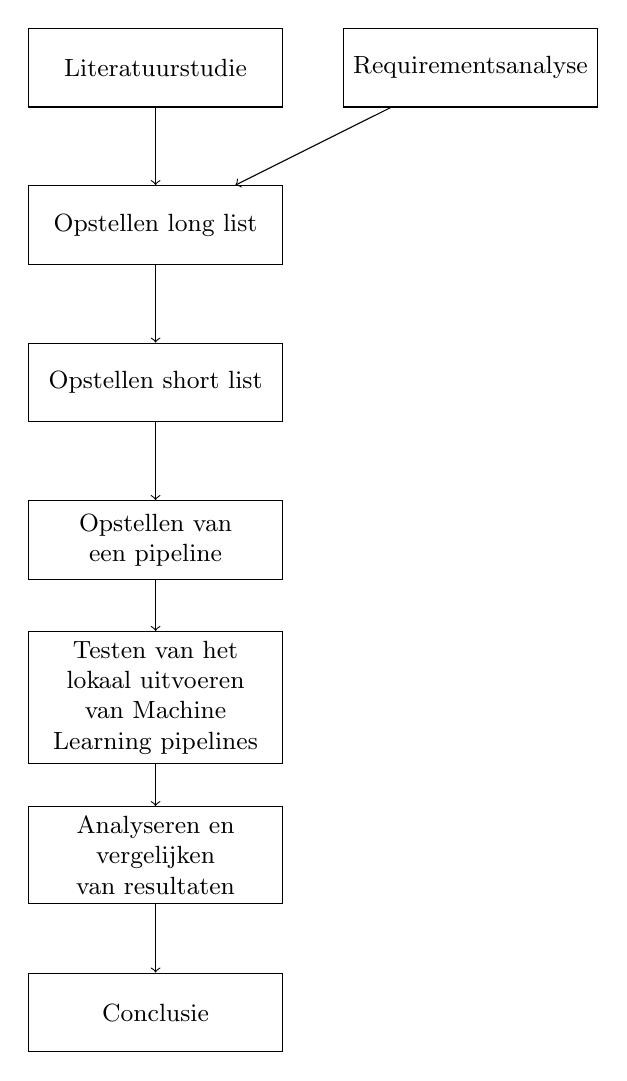
\begin{tikzpicture}[node distance=2cm, every node/.style={font=\small}]
  \node (pro0) [rectangle, draw, minimum width=3cm, minimum height=1cm, text centered, text width=3cm] {Literatuurstudie};
  \node (pro8) [rectangle, draw, minimum width=3cm, minimum height=1cm, text centered, text width=3cm, right of=pro0, xshift=2cm] {Requirements\-analyse};
  \node (pro1) [rectangle, draw, minimum width=3cm, minimum height=1cm, text centered, text width=3cm,below of=pro0] {Opstellen long list};
  \node (pro3) [rectangle, draw, minimum width=3cm, minimum height=1cm, text centered, text width=3cm, below of=pro1] {Opstellen short list};
  \node (pro4) [rectangle, draw, minimum width=3cm, minimum height=1cm, text centered, text width=3cm, below of=pro3] {Opstellen van een pipeline};
  \node (pro5) [rectangle, draw, minimum width=3cm, minimum height=1cm, text centered, text width=3cm, below of=pro4] {Testen van het lokaal uitvoeren van Machine Learning pipelines};
  \node (pro6) [rectangle, draw, minimum width=3cm, minimum height=1cm, text centered, text width=3cm, below of=pro5] {Analyseren en vergelijken van resultaten};
  \node (pro7) [rectangle, draw, minimum width=3cm, minimum height=1cm, text centered, text width=3cm, below of=pro6] {Conclusie};

  \draw [->] (pro0) -- (pro1);
  \draw [->] (pro1) -- (pro3);
  \draw [->] (pro3) -- (pro4);
  \draw [->] (pro4) -- (pro5);
  \draw [->] (pro5) -- (pro6);
  \draw [->] (pro6) -- (pro7);
  \draw [->] (pro8) -- (pro1);
\end{tikzpicture}

%% TODO: In dit hoofstuk geef je een korte toelichting over hoe je te werk bent
%% gegaan. Verdeel je onderzoek in grote fasen, en licht in elke fase toe wat
%% de doelstelling was, welke deliverables daar uit gekomen zijn, en welke
%% onderzoeksmethoden je daarbij toegepast hebt. Verantwoord waarom je
%% op deze manier te werk gegaan bent.
%% 
%% Voorbeelden van zulke fasen zijn: literatuurstudie, opstellen van een
%% requirements-analyse, opstellen long-list (bij vergelijkende studie),
%% selectie van geschikte tools (bij vergelijkende studie, "short-list"),
%% opzetten testopstelling/PoC, uitvoeren testen en verzamelen
%% van resultaten, analyse van resultaten, ...
%%
%% !!!!! LET OP !!!!!
%%
%% Het is uitdrukkelijk NIET de bedoeling dat je het grootste deel van de corpus
%% van je bachelorproef in dit hoofstuk verwerkt! Dit hoofdstuk is eerder een
%% kort overzicht van je plan van aanpak.
%%
%% Maak voor elke fase (behalve het literatuuronderzoek) een NIEUW HOOFDSTUK aan
%% en geef het een gepaste titel.

